\documentclass{article}
\usepackage{final_project,times}
\newcommand{\comment}[1]{}
\usepackage[numbers]{natbib}
\usepackage{booktabs}
\usepackage{bbm}
\usepackage{float}
\usepackage{amsmath,amsthm,amsfonts,amssymb,amscd}
\usepackage{array}
%\usepackage{floatrow}
\usepackage{mathptmx}
\usepackage{alltt}
\usepackage{textcomp}
\newcolumntype{M}{>{$}c<{$}}
\usepackage{url}
\usepackage{graphicx}
\usepackage{caption}
\usepackage{subcaption}

%\documentstyle[nips12submit_09,times,art10]{article}


\title{Analyzing Market Cycles with Persistent Homology}


\author{
Aashiq Dheeraj, Christian Drappi \\
Math 412, Prof. John Harer \\
Department of Mathematics, Duke University
}

\newcommand{\fix}{\marginpar{FIX}}
\newcommand{\new}{\marginpar{NEW}}

\nipsfinalcopy

\begin{document}

\large

\maketitle

\begin{abstract}
We examine stock price data from four major European indices between 1991 and 1998 using the machinery of Persistent Homology. First, we examine the topological structure of the stocks' logarithmic returns. Secondly, we propose a method to predict future returns with homology, inspired by Mandelbrot's fractal theory of the markets. Finally, we compare market behavior over different periods of time by clustering persistence diagrams.
\end{abstract}

\newpage

\section{Introduction}
Traders have different theories on price movements, derived from realms as diverse as stochastic processes and vedic astrology. Two of these include the Efficient Market Hypothesis and Elliot Wave Theory. The efficient market hypothesis holds that stock prices are a martingale, with an expected log return rate of 0 in the short run \cite{samuelson1965}. This view is popular among economists and mathematicians who can use this property to prove important results. 

However, many traders have had success using technical analysis-- the inference of future price movements from past patterns. The Elliot Wave Principle is one such technique, which suggests that the market oscillates between an optimistic, motive phase and a pessimistic, corrective phase at every time scale \cite{frost2005}. Mandelbrot published a seminal work on the self-similar, repeating structure of the markets \cite{mandelbrot2005}. He analyzes the Joseph Effect, the idea that price movements follow from larger trends, even quantifying its existence. He then goes on to assert the existence of this effect at multiple time-scales, all the way down.  While we are sympathetic towards the efficient markets view, we decided to investigate the existence and predictive power of repetitive structure in the market at different time scales. In other words, given data for the past $n$ days, we want to predict price movements over the next $n$ days. To do this, we want to identify the historical $n$-day period, $T_i$,  that most resembles the current market environment and use $T_{i+1}$ for prediction.


\section{Data}
The data consists of prices of four major European indices - the DAX, SMI, CAC and FTSE - between 1991 and 1998. The data comes from R's built in ``datasets'' package \cite{rprog}.

In mathematical theories of finance, price is not the quantity of interest, as it is not directly comparable between securities. Rather, financiers are more interested in the change in the logarithm of the price – the “log returns”. Therefore, we transformed our price data to log returns data. To do this, we divided the price from the $(t+1)$st time step by the price from the $t$th time step, and then computed its logarithm.

One convenience of using log returns is that they are additive. So, if we wished to understand topological structure in monthly log returns, we could simply add the log returns for each month, and compute persistence. In addition, if prices follow a Geometric Brownian Motion as is often assumed, the log returns will be normally distributed.

\newpage

\section{Methods}

\subsection{Persistent Homology over Log Returns}
We can compute persistence for the log returns data. The computation of the 0-dimensional diagram is similar to a general-purpose clustering algorithm. Persistent structure would suggest the existence of several distinct archetypes with characteristic return profiles. Returns on a given day could be described by one of these. The computation of the 1-dimensional persistence tells us about the existence of holes in the data. This corresponds to the impossibility of certain return profiles.

We have too many points to blindly compute persistence over all length scales. We can generate the pairwise distance for 100,000 randomly selected days to get a sense for the characteristic length scales at which features might appear. We expect that most features should begin to appear before we connect each data point to a full half of the remaining data. We set the maximum edge length close to but below the median and proceed. The algorithm still takes an inordinate amount of time, so we can sample 200 points and compute persistence for these. This sampling is only done for exploratory analysis of the daily log-returns considered as a whole, and not for the chunked data considered below.

We used the ``phom'' package in R to compute persistence for point clouds \cite{phom}. For distance matrices we used the RCA1 library provided in class \cite{TDA}. Both these methods use algorithms found in \cite{de2011}. Points in a point-cloud are thickened over time and a simplicial complex is built up by adding intersections. The Rips construction is used, so a simplex is added once its boundary is added.

%% FIX THIS
\subsection{Wasserstein Distance}

We can separate the data into $n$-day chunks and compute the 1-dimensional persistence diagrams for each chunk, to characterize the cyclical behavior. The Wasserstein distance gives a metric for comparing persistence diagrams. Let $X$ and $Y$ be two persistence diagrams. A persistence diagram consists of a sequence of birth and death time pairs along with the infinitely many points on the diagonal where birth equals death . Let $\eta$ denote a perfect matching between $X$ and $Y$, a bijection where points are matched up wherever possible and leftovers are sent to the closest point on the diagonal. Then the $q^{\text{th}}$ Wasserstein distance is given by 
\[
W_q(X,Y) = \left[ \text{inf}_{\eta:X \rightarrow Y} \sum_{x \in X} || x  - \eta(x) ||^q_\infty \right]^{\frac{1}{q}}
\]

By computing the pairwise Wasserstein distance between chunks in the training set, we arrive at an $\lfloor \frac{1833}{n} \rfloor$ -dimensional kernel, denoted $W_n$. We used Dmitriy Morozov's Dionysus library for computation \cite{morozov2012}.

\newpage

\subsection{Method of Closest Diagram}
One problem that all financiers wish they could solve is predicting future stock returns. Inspired by Mandelbrot's insistence on repetitive, self-similar structure, we sought to understand how the topological structure of log returns could predict future returns. We divided log returns into $c$ chunks of size $n$. Then we computed persistence diagrams for each chunk. Using the Dmitriy Morozov's implementation of the Wasserstein distance in Dionysus \cite{morozov2012}, we computed a $c \times c$ matrix of distances between diagrams that represent each chunk.

Then, we split our data into a training set and a test set. We trained on data from years 1991-1996 and tried to predict data from years 1997-1998. For each chunk in the test set, $i$, we looked at the chunk right before it, $i-1$. Using the $c \times c$ matrix of persistence diagrams, we located the chunk “most similar” to chunk $i-1$, call it $j-1$. Then we said the log returns of chunk $i$ should mirror the log returns of chunk $j$, as they shared similar “market shape” in the previous time period. So, our method of closest diagrams predicted the returns of chunk $i$ with those of chunk $j$. 


\subsection{Persistence of persistence diagrams}
Fractal theories of the market maintain that cyclical structure is evident at every time scale. We can compute persistence on the set of persistence diagrams for an $n$-day partition of the data using $W_n$ as an explicit distance matrix. This gives a notion of structure among chunks considered as individual objects, elucidating the potential fractal structure of one-cycles.


\section{Interpretation}

\subsection{General persistence over log returns}

The distribution of pairwise distances is plotted below. It seems to be a positively skewed, unimodal distribution with a median of 0.02. Setting the maximum edge length to 0.015, we expect to capture most important features while saving on time and avoiding addition of unimportant simplices. The phom algorithm still takes too long, so we sample 200 random data from the log returns and run persistence on these.

\begin{figure}
\begin{center}
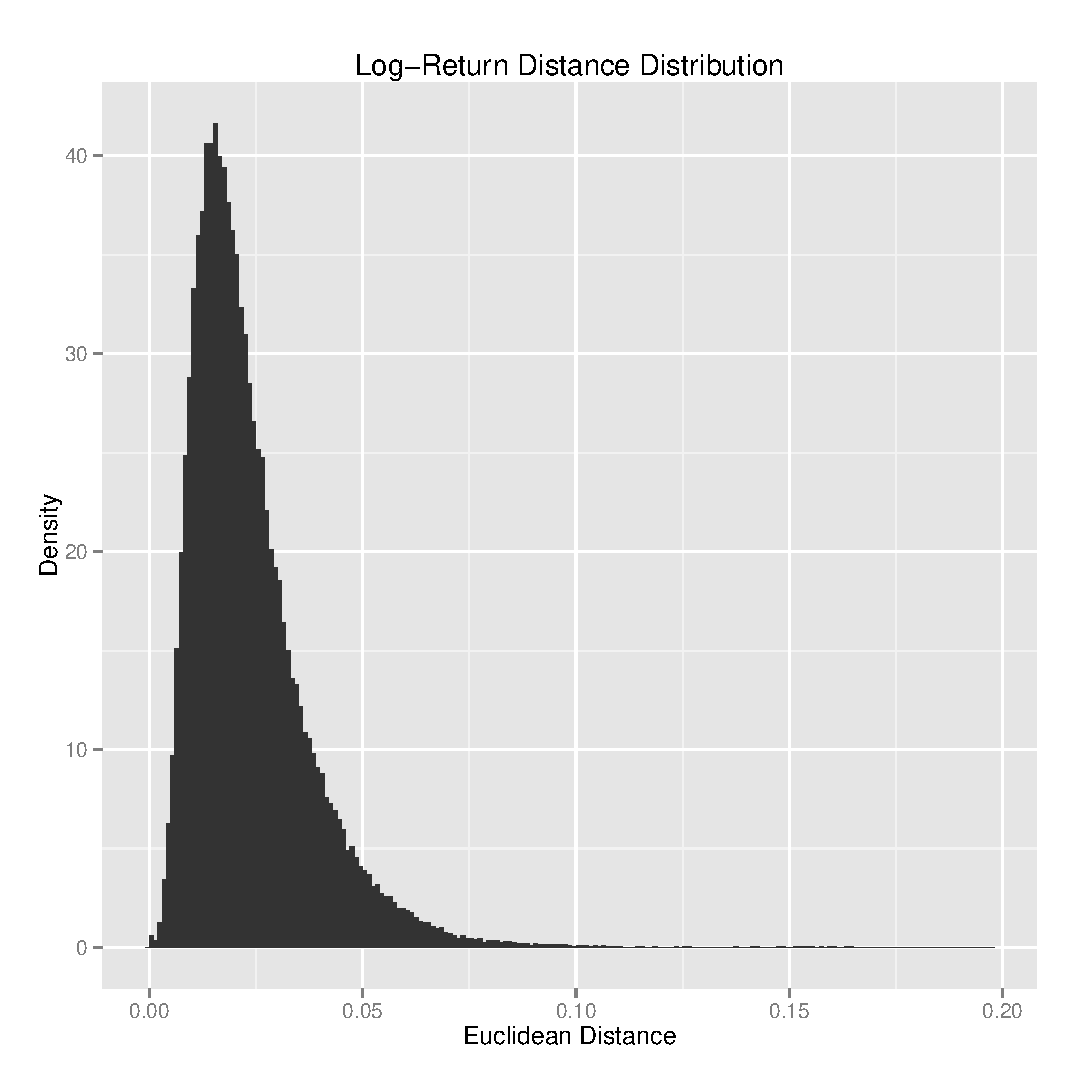
\includegraphics[width = 3.5 in, height = 3.5 in]{globplots/lr-dist}
\caption{The log-returns for a  day are $r \in \mathbb{R}^4$. The distance between two days is given by the Euclidean metric.}
\label{lrdist}
\end{center}
\end{figure}


\begin{figure}
\centering
\begin{subfigure}[htbp]{0.45 \textwidth}
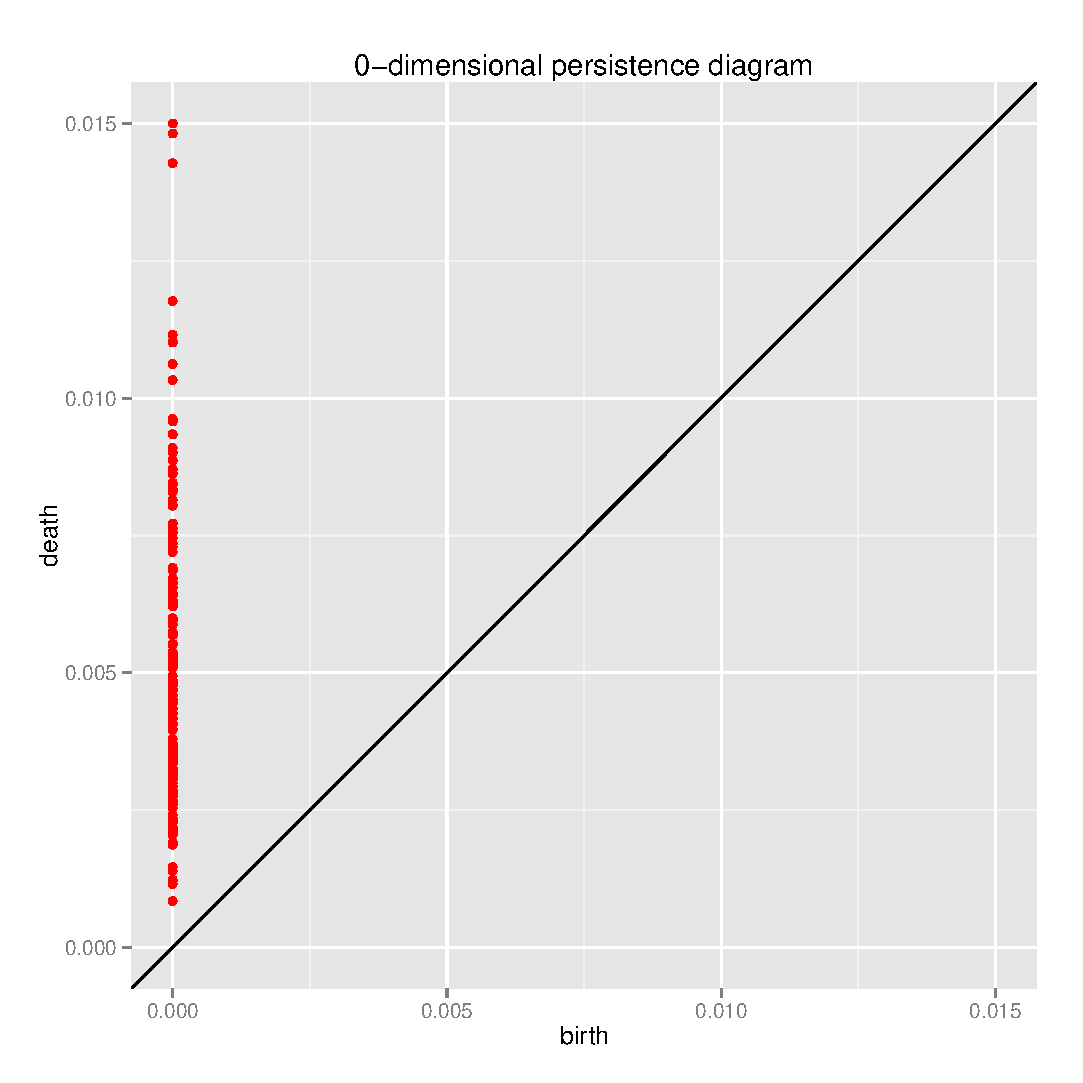
\includegraphics[width = \linewidth]{globplots/rlr-200-0-f15e-3}
\caption{We have a few clusters}
\label{lr0}
\end{subfigure}
~
\begin{subfigure}[htbp]{0.45 \textwidth}
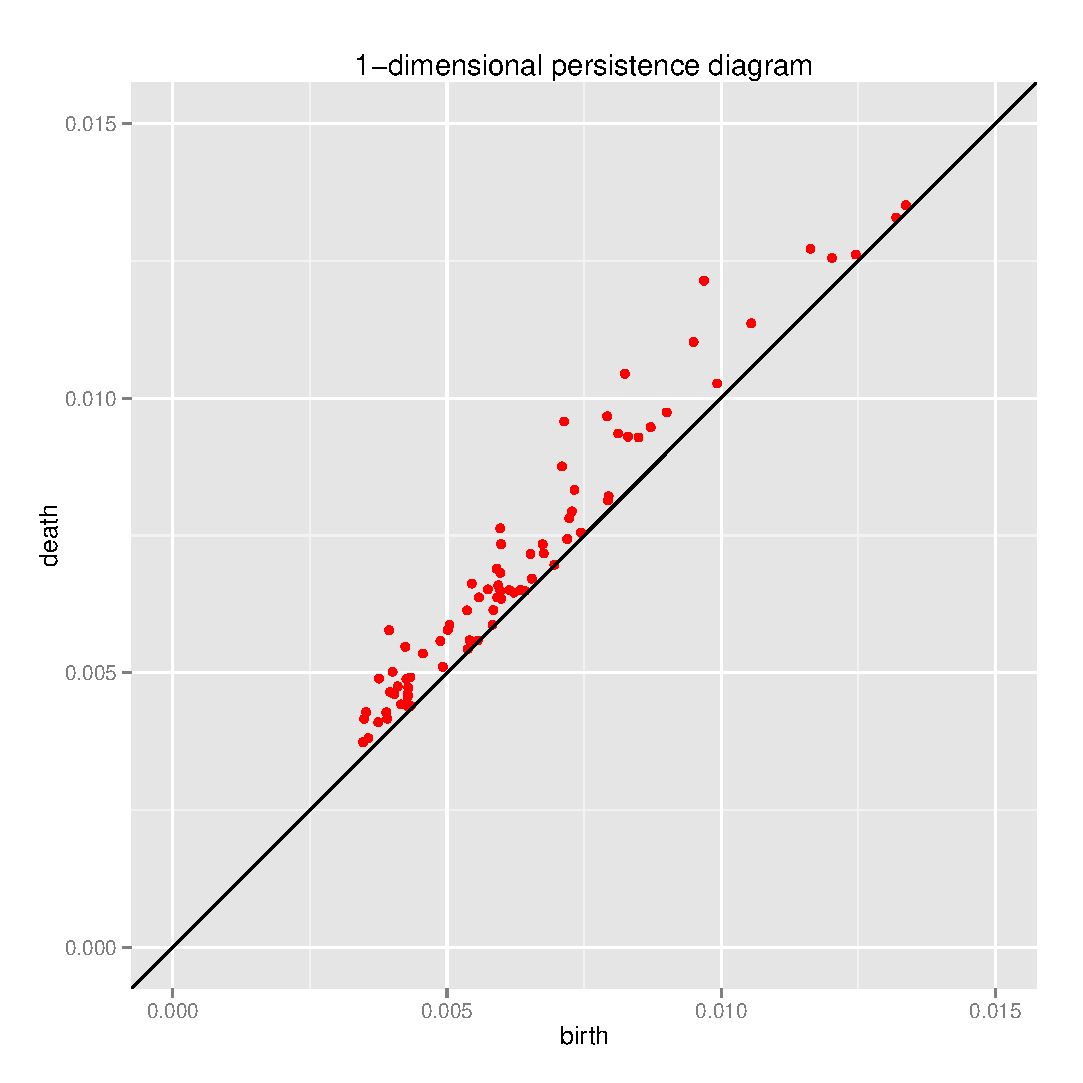
\includegraphics[width = \linewidth]{globplots/rlr-200-1-f15e-3}
\caption{There are no persistent 1-cycles}
\label{lr1}
\end{subfigure}
\label{lr}
\end{figure}

The structure of this data implies that there are a set of characteristic configurations that the return profile for the four indices can take. As major stock indices are highly correlated, this is unsurprising. The existence of structure is interesting, but cannot itself be used for prediction, which we address below.


\newpage

\subsection{Predicting Returns using Market Cycles}
To measure the predictive success of our closest diagram method, we computed the root-mean-square error of prediction (RMSE) on our test set. The formula for RMSE is: 

\begin{center}{
$\mathrm{RMSE}(P) = \sqrt{\frac{1}{T} \, \sum\limits_{t=1}^T [x_t - P(x_t)]} $
}\end{center}

Where  $\{x_t\}$ is our test set of size $T$, and $P(\cdot)$ is the function that returns a prediction.

To benchmark our results, we also computed the RMSE of the method that predicts the same price as before. That is, the prediction if the log returns were truly a martingale. Our results are listed in the table below.

\begin{center}{
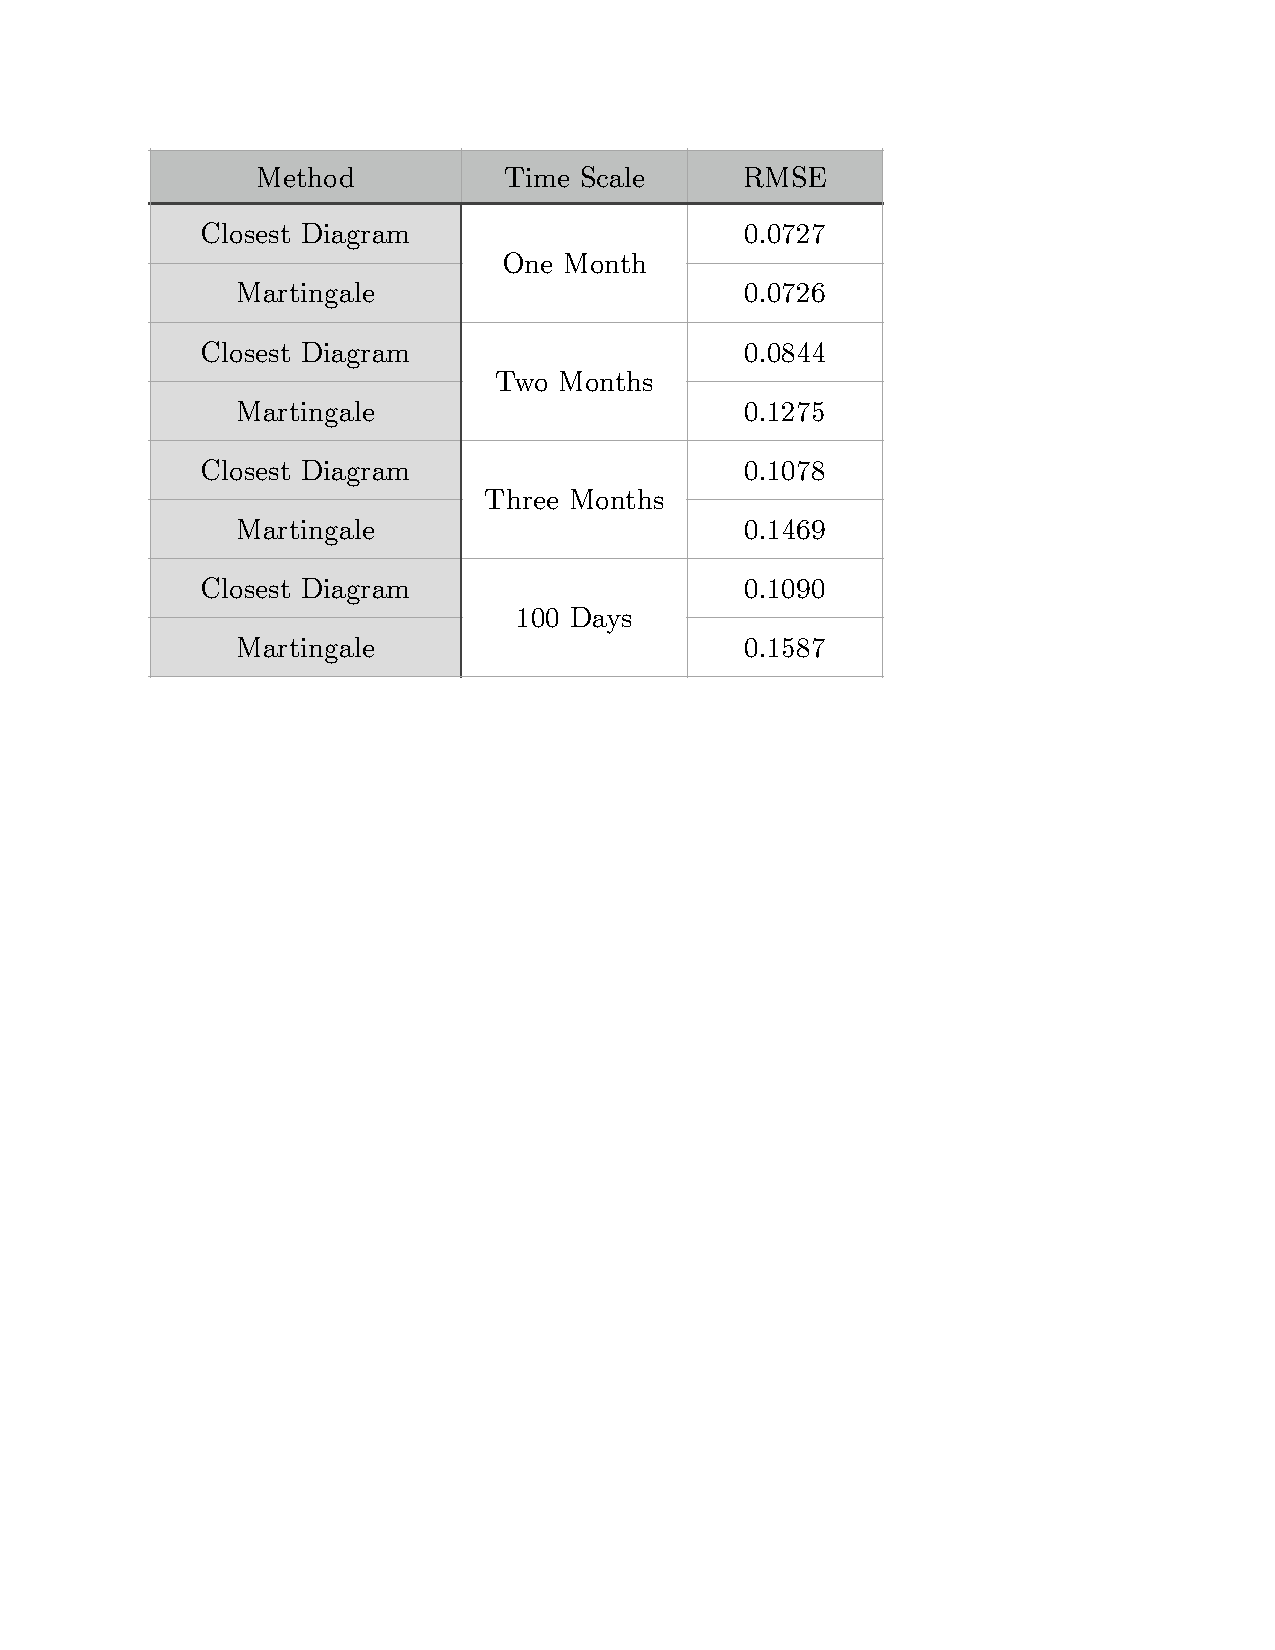
\includegraphics[width=0.75\textwidth]{rmse}
}\end{center}

Our method outperforms the null hypothesis (stock price is a martingale) at every time-scale except one month. Since we don’t have as much data as we would have liked, we are not confident that this is a pattern, but it is worth further investigation.

\subsection{Similarity over Time Scales}
Computing persistence between chunks resulted in trivial 0-D diagrams and slightly less trivial 1-D diagrams. The latter plots are shown on the following page.

\newpage

\begin{figure}
\centering
\begin{subfigure}[htbp]{0.49 \textwidth}
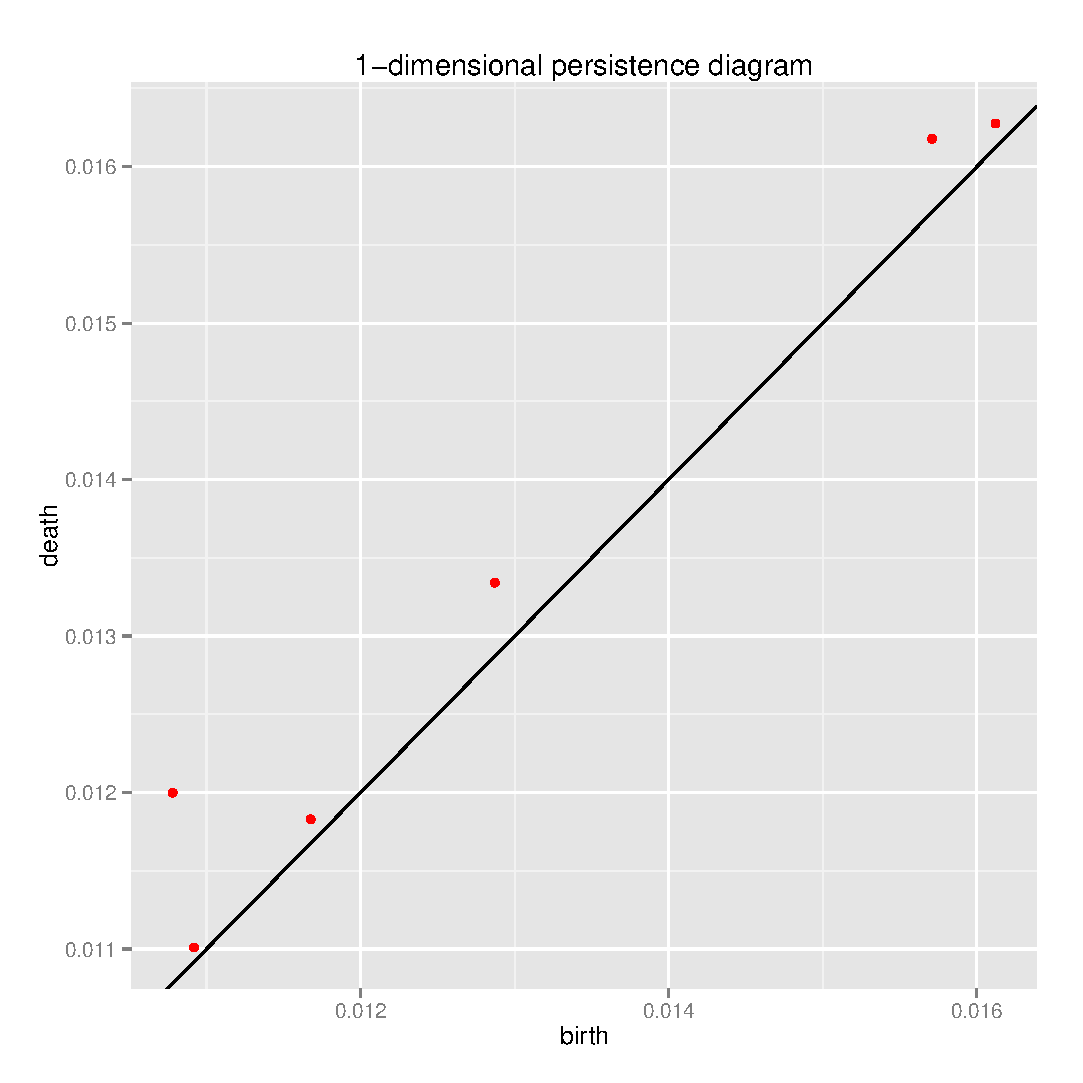
\includegraphics[width = \linewidth]{psqplots/p2-1-90}
\caption{$n = 30$}
\label{p2-1-30}
\end{subfigure}
~
\begin{subfigure}[htbp]{0.49 \textwidth}
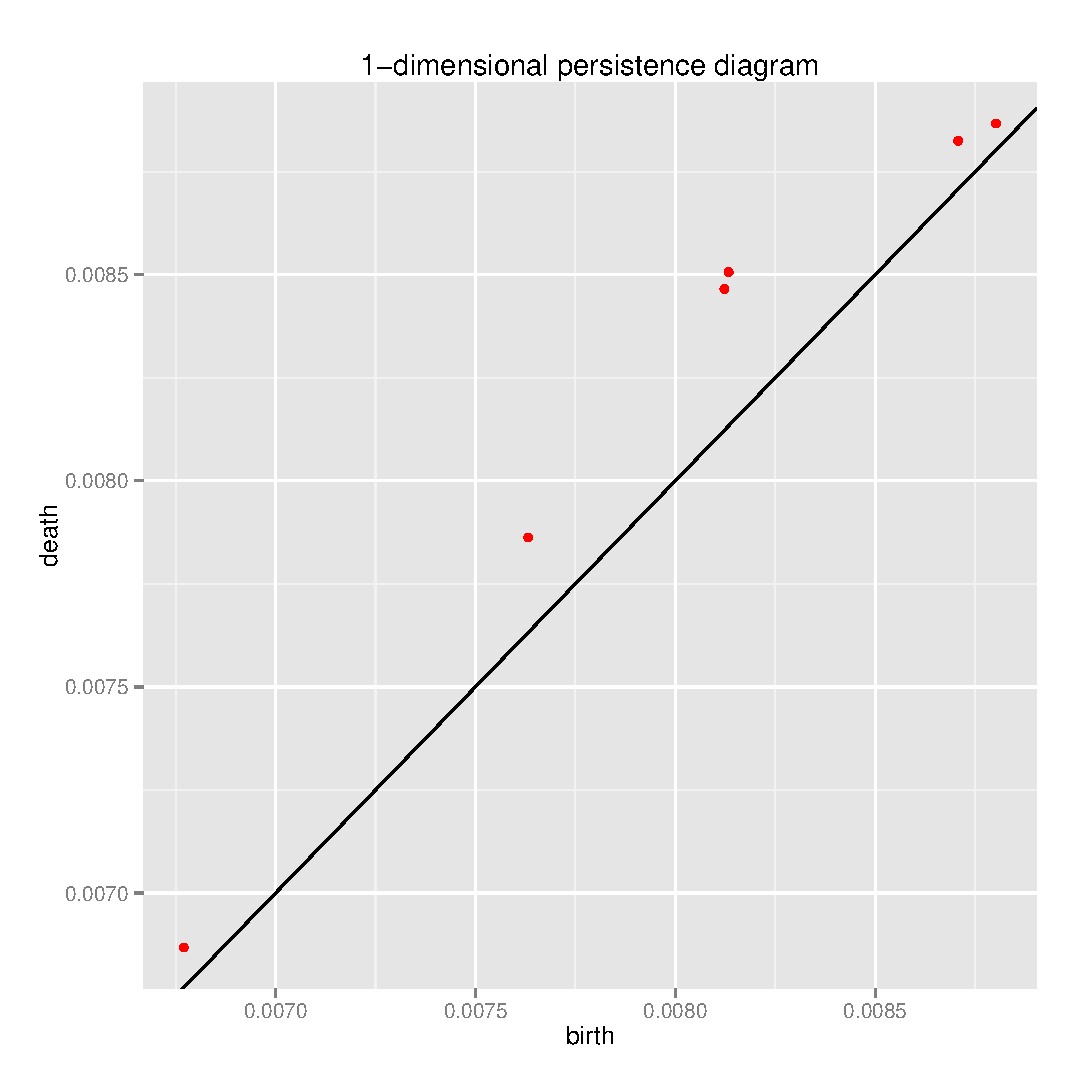
\includegraphics[width = \linewidth]{psqplots/p2-1-60}
\caption{$n = 60$}
\label{p2-1-60}
\end{subfigure}
\begin{subfigure}[htbp]{0.49 \textwidth}
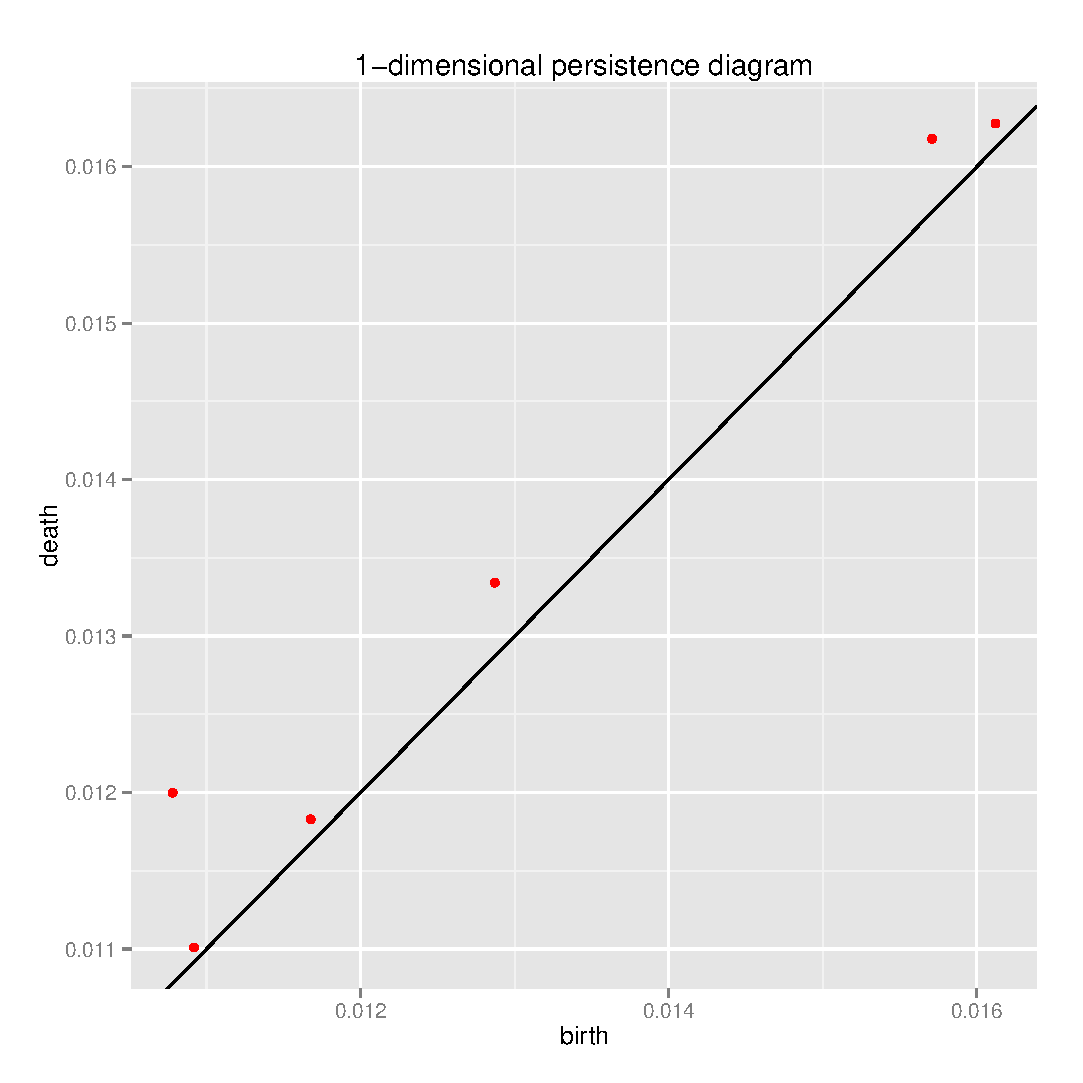
\includegraphics[width = \linewidth]{psqplots/p2-1-90}
\caption{$n = 90$}
\label{p2-1-90}
\end{subfigure}
\label{p2-1}
\caption{1-D Persistence for Various Chunk Sizes}
\end{figure}
\section{Conclusion}
\vspace{-15mm}
An analysis of log-returns data shows some persistent 0- and 1-dimensional clustering at a characteristic length scale of around 0.015. A small Wasserstein distance between the persistence diagrams for two distinct time periods $t_i$ and $t_j$ seems to predict increased correlation between asset returns over the subsequent time periods $t_{i+1}$ and $t_{j+1}$. The Wasserstein kernel acts as a topologically invariant auto-correlation. If confirmed, this pattern would be in violation of the efficient market hypothesis in its weakest form, as this amounts to a sophisticated form of technical analysis. The use of the computed Wasserstein kernel as a distance matrix does not yield persistent homology for any chunk size.

\section{Future Investigations}

\subsection{More data, different markets}
Our closest diagram method did okay, but we would like to see it trained and tested on more data. We might instead want to try this on data with less correlation, too. A good example of this would be foreign exchange rates, which have more “zero sum” behavior than European indices.

\subsection{Kernel-Based Methods}
We have computed a kernel based on Wasserstein distance, and this can be used in a number of machine learning algorithms. Suppose we want to discriminate between winning, losing, and constant months. We can use our kernel to train a support vector machine, projecting our data into a higher-dimensional space where the three classes are linearly separable. Alternatively, we can employ PCA to reduce the dimensionality of the data. In this way, persistence diagrams might be characterized by a few eigendiagrams.


\subsection{Options pricing}
In our investigation thus far, we have only considered this 4-dimensional data on European stock indices. The 4 indices are highly correlated, potentially accounting for the dearth of interesting structure. Alternatively, we might look at prices of options. American options give the holder the right but not the obligation to buy or sell a given security on or before a given date for a specified price. The value of an option is a function of the price of the underlying, the volatility, and the interest rate. These quantities are less correlated than the major  European indices, but are related in interesting ways in different market climates. Thus, we expect there to be more interesting topological structure.

\subsection{Explicit Time-Dependence}
We treated this time-series by chunking up the data and seeing if past time-series have predictive power. Alternatively, we could have modeled time explicitly. In this case, one-cycles can be directly interpreted as periodic orbits-- enabling comparison to models like Elliot waves. Furthermore, we can look at different delays to see the geometry of potential attractors \cite{muldoon1993}. The success of the Wasserstein kernel in prediction for different chunk sizes suggests potential choices of delay.

\newpage

\nocite{*}
\bibliography{final_project}
\bibliographystyle{ieeetr}


\end{document}